\documentclass[11pt, letterpaper]{article}
\usepackage[top=1in, bottom=1in, left=1in, right=1in]{geometry}


% Math, graphics, and bibliography
\usepackage{amsmath,amssymb,amsfonts,mathrsfs}
\usepackage{graphicx}
\usepackage[round,numbers,sort&compress]{natbib}
\renewcommand{\bibnumfmt}[1]{#1.}
% \usepackage[square,sort,comma,numbers]{natbib} % my preferred formatting

% My preferred fonts
\usepackage[T1]{fontenc}
\usepackage{lmodern}
\usepackage[sc]{mathpazo}

% For fancier fractions and figure captions
\usepackage[labelfont={bf}, margin=1cm]{caption}
\usepackage{units}

% For model float
\usepackage{float}
\newfloat{model}{thp}{lop}
\floatname{model}{Model}
\floatstyle{plaintop}
\restylefloat{model}
\usepackage{supertabular}
\usepackage{booktabs}

\begin{document}

\begin{model}
\caption{Adapted from Nov\'{a}k \& Tyson, 2008 \cite{Novak2008}. Model used for
ARC demonstrations in Figs. 1-3, S1 ($P=4$) and Fig. S2, Movies S1 \& S2
($P=2$).}
  \centering
\begin{align*}
  \frac{dX}{dt} &= \frac{1}{1 + Y} - X \\
  \frac{dY}{dt} &= k_t \; X - k_d \; Y - \frac{Y}{\alpha_0 + \alpha_1 \; Y +
  \alpha_2 Y^2}
\end{align*}
  
\tablehead{\toprule Parameter & Value\\\midrule}
\begin{supertabular}{rl}
$k_t$ & 20 \\
$k_d$ & 1  \\
$P$   & 4 (or 2)  \\
\bottomrule\end{supertabular}\hspace{3ex}
\begin{supertabular}{rl}
$\alpha_0$ & 0.005 \\
$\alpha_1$ & 0.05  \\
$\alpha_2$ & 0.1   \\
\bottomrule\end{supertabular}
\end{model}

\begin{model}
\caption{Hirota {\itshape et al.} 2012 \cite{Hirota2012}. A more detailed model
of circadian rhythms used for simulations in Figs. 4-5.}
  \centering
\begin{align*}
\frac{d\,\mathit{p}}{dt} &= \frac{- \mathit{p} \cdot \mathit{vdp}}{\mathit{kdp} + \mathit{p}} + \frac{\mathit{vtp}}{\mathit{knp} + \left(\mathit{C1n} + \mathit{C2n}\right)^{3}}\\
\frac{d\,\mathit{c1}}{dt} &= \frac{- \mathit{c1} \cdot \mathit{vdc1}}{\mathit{c1} + \mathit{kdc1}} + \frac{\mathit{vtc1}}{\mathit{knc1} + \left(\mathit{C1n} + \mathit{C2n}\right)^{3}}\\
\frac{d\,\mathit{c2}}{dt} &= \frac{- \mathit{c2} \cdot \mathit{vdc2}}{\mathit{c2} + \mathit{kdc1}} + \frac{\mathit{vtc2}}{\mathit{knc1} + \left(\mathit{C1n} + \mathit{C2n}\right)^{3}}\\
\frac{d\,\mathit{P}}{dt} &= - \mathit{C1} \cdot \mathit{P} \cdot \mathit{vaC1P} + \mathit{C1n} \cdot \mathit{vdC1P} - \mathit{C2} \cdot \mathit{P} \cdot \mathit{vaC1P} + \mathit{C2n} \cdot \mathit{vdC1P} - \frac{\mathit{P} \cdot \mathit{vdP}}{\mathit{P} + \mathit{kdP}} + \mathit{ktxnp} \cdot \mathit{p}\\
\frac{d\,\mathit{C1}}{dt} &= - \mathit{C1} \cdot \mathit{P} \cdot \mathit{vaC1P} - \frac{\mathit{C1} \cdot \mathit{vdC1}}{\mathit{C1} + \mathit{kdC1}} + \mathit{C1n} \cdot \mathit{vdC1P} + \mathit{c1}\\
\frac{d\,\mathit{C2}}{dt} &= - \mathit{C2} \cdot \mathit{P} \cdot \mathit{vaC1P} - \frac{\mathit{C2} \cdot \mathit{vdC2}}{\mathit{C2} + \mathit{kdC1}} + \mathit{C2n} \cdot \mathit{vdC1P} + \mathit{c2}\\
\frac{d\,\mathit{C1n}}{dt} &= \mathit{C1} \cdot \mathit{P} \cdot \mathit{vaC1P} - \mathit{C1n} \cdot \mathit{vdC1P} - \frac{\mathit{C1n} \cdot \mathit{vdCn}}{\mathit{C1n} + \mathit{C2n} + \mathit{kdCn}}\\
\frac{d\,\mathit{C2n}}{dt} &= \mathit{C2} \cdot \mathit{P} \cdot \mathit{vaC1P} - \frac{\mathit{C2n} \cdot \mathit{MC2n} \cdot \mathit{vdCn}}{\mathit{C1n} + \mathit{C2n} + \mathit{kdCn}} - \mathit{C2n} \cdot \mathit{vdC1P}\\
\end{align*}
  
\tablehead{\toprule Parameter & Value\\\midrule}

\begin{supertabular}{rl}
$vtp $  & 0.195   \\
$vtc1$  & 0.131   \\
$vtc2$  & 0.114   \\
$knp $  & 0.425   \\
$knc1$  & 0.259   \\
$vdp $  & 0.326   \\
$vdc1$  & 0.676   \\
\bottomrule\end{supertabular}\hfil
\begin{supertabular}{rl}
$vdc2$ & 0.608   \\
$kdp $ & 0.0115  \\
$kdc1$ & 1.15    \\
$vdP $ & 2.97    \\
$vdC1$ & 0.0338  \\
$vdC2$ & 1.52    \\
$vdCn$ & 1.69    \\
\bottomrule\end{supertabular}\hfil
\begin{supertabular}{rl}
$MC2n $ & 2.02    \\
$kdP  $ & 0.101   \\
$kdC1 $ & 3.32    \\
$kdCn $ & 0.0526  \\
$vaC1P$ & 0.0406  \\
$vdC1P$ & 0.00175 \\
$ktxnp$ & 3.0     \\
\bottomrule\end{supertabular}
\end{model}

\begin{model}
  \caption{The Oregonator model \cite{Field1974}, with parameters as presented
  in \cite{Gillespie1977}. Used in Fig.~S3 as an example of a limit cycle
oscillator using only mass-action kinetics.}

  The individual chemical reactions (used for stochastic simulation) are:
\begin{align*}
  X_1 + Y_2 &\xrightarrow{c_1} Y_1\\
  Y_1 + Y_2 &\xrightarrow{c_2} Z_1\\
  X_2 + Y_1 &\xrightarrow{c_3} 2Y_1 + Y_3\\
  2Y_1 &\xrightarrow{c_4} Z_2\\
  X_3 + Y_3 &\xrightarrow{c_5} Y_2
\end{align*}

These reactions can be converted to a standard ODE model, in which only the
intermediate variables $Y$ are considered, as:
\begin{align*}
  \frac{d\,\mathit{Y1}}{dt} &= \mathit{c1x1}\cdot\mathit{Y2} -
  \mathit{c2}\cdot\mathit{Y1}\cdot\mathit{Y2} + \mathit{c3x2}\cdot\mathit{Y1} -
  \mathit{c4}\cdot\mathit{Y1}^2\\
  \frac{d\,\mathit{Y2}}{dt} &= -\mathit{c1x1}\cdot\mathit{Y2} -
  \mathit{c2}\cdot\mathit{Y1}\cdot\mathit{Y2} + \mathit{c5x3}\cdot\mathit{Y3}\\
  \frac{d\,\mathit{Y3}}{dt} &= \mathit{c3x2}\cdot\mathit{Y1} -
  \mathit{c5x3}\cdot\mathit{Y3}
\end{align*}
  
\begin{center}
  \tablehead{\toprule Parameter & Value\\\midrule}
  \begin{supertabular}{rl}
    $\mathit{c1x1}$ & 2 \\
    $\mathit{c2}$ & 0.1 \\
    $\mathit{c3x2}$ & 104 \\
    $\mathit{c4}$ & 0.016 \\
    $\mathit{c5x3}$ & 26 \\
    \bottomrule\end{supertabular}
\end{center}
\end{model}


\renewcommand{\thefigure}{S\arabic{figure}}
\setcounter{figure}{0}

\begin{figure}[h!]
  \begin{center}
    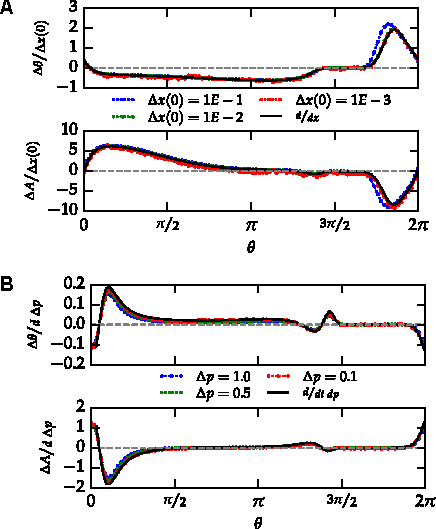
\includegraphics[width=.75\textwidth]{figures/figure_S1.pdf}
    \caption{{\bfseries Convergence of finite-difference and differential
    methods.} ({\bfseries A}) Perturbations of decreasing strength to the state
    of the oscillator result in phase and amplitude response curves that match
    the differential limit. ({\bfseries B}) Temporary perturbations of
    decreasing strength to a kinetic parameter. The duration of each
    perturbation is fixed to 0.2 radians. Finite difference approximations
    closely match the differential method, which is offset in phase by 0.1
    radians to account for the nonzero pulse duration.}
\end{center}
\end{figure}

\begin{figure}[h!]
  \begin{center}
    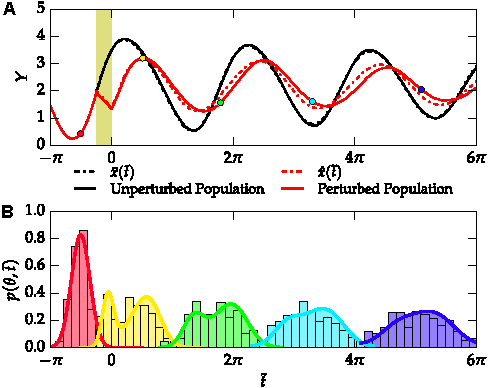
\includegraphics[width=.75\textwidth]{figures/figure_S2.pdf}
    \caption{{\bfseries Approximation of an explicit stochastic population by
    continuous methods.} ({\bfseries A}) A population of 225 stochastic
    oscillators was simulated using the Gillespie stochastic simulation
    algorithm (SSA), see Movie S1 and S2. The mean protein
    expression, $Y$, is plotted as a function of time. A $50\%$ reduction in
    the protein translation rate to each of the oscillators is applied from
    $\hat{t} = -\nicefrac{\pi}{4} \to 0$, resulting in both single-cell and
    population-level amplitude change (red solid line). This population is
    approximated by the continuous methods described in this manuscript, in
    which the decay parameter $d=0.025$ is estimated to match the
    stochastic-induced desynchrony of the control population (black solid
    line). The initial standard deviation $\sigma_0 = 0.48$ is similarly
    matched to the stochastic population. The resulting predicted unperturbed
    and perturbed trajectories, $\bar{x}(\hat{t})$ and $\hat{x}(\hat{t})$
    respectively, closely match the stochastically modeled values.  ({\bfseries
    B}) Phase histograms for the stochastic population are shown at several
    phases, both before and after the desynchronizing perturbation.  Phase
    probability-density functions for the continuous approximation are also
    shown, with close agreement between stochastic and continuous simulations.
    This close approximation validates the use of ODE models and
  phase-diffusion populations in deriving amplitude and phase-response behavior
for networks of uncoupled cells.}
\end{center}
\end{figure}

\begin{figure}[h!]
  \begin{center}
    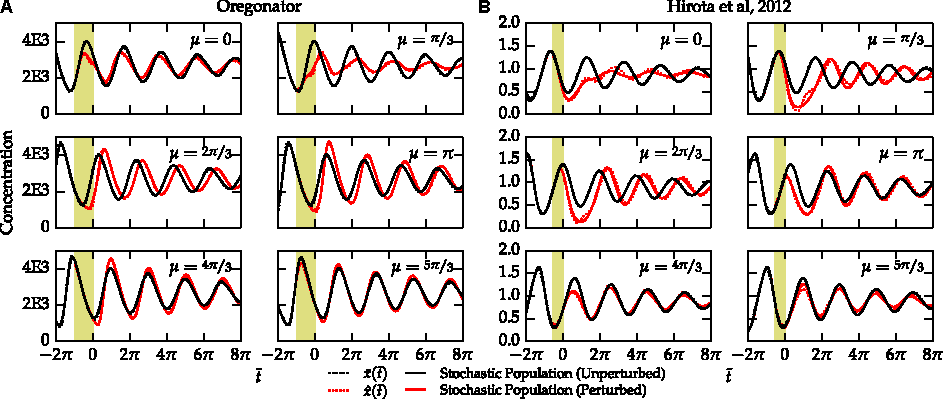
\includegraphics[width=\textwidth]{figures/figure_S3.pdf}
    \caption{{\bfseries Validation of continuous methods with alternate
    models.} ({\bfseries A}) The Oregonator model (Model 3) was tested as an
    example of a mass-action limit cycle oscillator. A population of 2000
    oscillators was perturbed at size different mean phases, $\mu$, by
    increasing the $\mathit{c2}$ parameter by $50\%$ for $d=\pi$ (highlighted
    region). Only the average $\mathit{Y2}$ variable is plotted. ({\bfseries
    B}) The model described in \cite{Hirota2012} (Model 2) was similarly tested
    at a variety of mean phases by reducing the $\mathit{vdp}$ parameter by
    $28.5\%$ and plotting the resulting $\mathit{c2}$ state variable (as in
    Fig.~5). Parameters for the continuous approximations were found by
    estimating the phase, initial standard deviation, period, and phase
    diffusivity of the control population. Good agreement is seen between the
  continuous and stochastic simulations, indicating the proposed method is
suitable for predicting the population-level responses for a variety of model
types.}
\end{center}
\end{figure}

\clearpage
{\bfseries Movie S1:} Stochastic simulation of a two-state limit
cycle oscillator. A population of 225 stochastic oscillators was simulated
using the Gillespie stochastic simulation algorithm (SSA). The deterministic
limit cycle, $x^\gamma(\hat{t})$, is shown in black (left), and the current
location of individual stochastic oscillators are shown by green dots. The
population average, plotted in both the state (left) and time (right) domains,
is shown in red. Stochastic noise drives the population to gradually
desynchronize, resulting in damped oscillations of the average protein level.
\\[2ex]

{\bfseries Movie S2:} Perturbation to a population of stochastic
oscillators. The population of oscillators is perturbed by a $50\%$ reduction
in the protein translation rate to each of the oscillators from $\hat{t} =
-\nicefrac{\pi}{4} \to 0$ (yellow frames), resulting in both single-cell and
population-level amplitude change. The oscillators quickly recover to the limit
cycle (single-cell level amplitude change), but the population is left
desynchronized (population-level amplitude change).

\renewcommand{\refname}{Supporting References}
\bibliographystyle{biophysj.bst}
\bibliography{condensed_library.bib}
\end{document}
